% =====================================================================
% Chapter 4 -- Proposed Methodology (file chapter_5.tex; title set in main.tex:135)
% Plan: thesis_tools/planning/CH4_METHODOLOGY_PLAN.md
% Every number carries "% src: <path> :: <field or line>". Collaborator files are read at
% the pinned commit 16def2de (git show 16def2de:<path>). Owner files are on asix @ e917ecd3
% plus the working tree. Lab-PC values come from the local caches under audit/cache/labpc/
% and audit/p17/labcache/, and are re-checked on the lab PC in the final verification step.
% Citation pages were checked against papers/*.pdf on 2026-09-24 (scratchpad ch4_citations.md); papers with no PDF are cited without a page.
% =====================================================================

\label{ch:method}
This chapter describes the method as one pipeline. It starts from persona prompts and ends with detection scores on eleven evaluation datasets, plus a twelfth, wording-controlled set scored separately.
Section~\ref{sec:m-overview} gives the whole design. Section~\ref{sec:m-spec} specifies the model, the persona coordinates, the features, the probes and the controls. Section~\ref{sec:m-built} describes what we built with the pipeline: new persona banks, new evaluation datasets and new evaluation tools.
Section~\ref{sec:m-data} covers the evaluation data and how we prepared it. Section~\ref{sec:m-impl} covers the evaluation protocols, the statistics and the implementation.

% ---------------------------------------------------------------------
\section{Design Process or Methodology Overview}
\label{sec:m-overview}

\begin{figure}[t]
\centering
\begin{tikzpicture}[
  node distance=4mm and 3mm,
  box/.style={draw, rounded corners=2pt, align=center, font=\footnotesize,
              minimum height=9mm, text width=21mm, fill=gray!8},
  arr/.style={-{Stealth[length=2mm]}, thick}]
\node[box] (bank) {Persona bank\\(roles, prompts,\\questions)};
\node[box, right=of bank] (roll) {Role-play\\rollouts};
\node[box, right=of roll] (judge) {Judge filter\\(score 0--3)};
\node[box, right=of judge] (vec) {Persona vectors\\(per layer)};
\node[box, below=of vec] (coord) {Contrasts and\\principal components};
\node[box, left=of coord] (feat) {Projection\\features};
\node[box, left=of feat] (eval) {Eval activations\\(11 datasets)};
\node[box, left=of eval] (score) {Zero-shot and\\trained detectors};
\draw[arr] (bank) -- (roll); \draw[arr] (roll) -- (judge); \draw[arr] (judge) -- (vec);
\draw[arr] (vec) -- (coord); \draw[arr] (coord) -- (feat); \draw[arr] (eval) -- (feat);
\draw[arr] (feat.south) |- ++(0,-4mm) -| (score.south);
\end{tikzpicture}
\caption{The persona-coordinate lie-detection pipeline, from persona bank to detector.}
\label{fig:m-pipeline}
\end{figure}

Figure~\ref{fig:m-pipeline} shows the pipeline. It follows the persona-coordinate method of \textcite[p.~3]{mahadik2026persona}, which builds on the role-vector recipe of \textcite[p.~3]{lu2026assistant}. We rebuilt every stage to run on a 70B model and added stages of our own. % pages: ch4_citations.md (checked against papers/*.pdf, 2026-09-24)

\begin{enumerate}
\item A \emph{persona bank} fixes a set of roles. Each role has system-prompt variants and a shared question set.
\item The subject model answers every question in every role. A judge model scores each answer for whether it displays the role, and we keep only the answers that do.
\item The mean activation over a role's kept answers is its \emph{persona vector}, one per layer.
\item Differences of group means give \emph{contrast directions}. Principal components of the persona vectors give \emph{persona coordinates}.
\item The detectors read evaluation activations through these directions. A detector either scores the projection directly, with no training (\emph{zero-shot}), or trains a small probe on it.
\end{enumerate}

Every stage writes its output to disk and can be resumed. % src: src/assistant_axis_ndif/8_coords_ndif.py :: 515 (chunk resume), 611 (failed sessions left for resume); collaborator deception_detection/acts_cache.py @16def2de (resumable per-example cache)

We use two implementations of the evaluation stage.
\begin{itemize}
\item \textbf{Pipeline~A} is our persona-coordinate implementation. Its main grid scores eleven datasets under every control of Section~\ref{sec:m-controls}. It scores the knowledge-matched HP-KR slice in a separate run. % src: audit/p17/labcache/expLB-resplit/run-crossgen/splits.json :: datasets (11); audit/cache/labpc/expLB-resplit/km/mean_L40_s42.json (12-dataset run)
\item \textbf{Pipeline~B} is built on the Liars' Bench detection code \parencite{kretschmar2025liars,goldowskydill2025detecting}. It scores the benchmark's datasets with the benchmark's own probe and metric.
\end{itemize}
The two share the persona vectors of Section~\ref{sec:m-built}. We describe both. Chapter~\ref{ch:results} states which one produced each result.

% ---------------------------------------------------------------------
\section{Preliminary Design or Design (Model) Specification}
\label{sec:m-spec}

\subsection{Subject model and compute}
\label{sec:m-model}

The subject model is Llama-3.3-70B-Instruct % src: src/assistant_axis_ndif/8_coords_ndif.py :: 669 (--model default)
\parencite{grattafiori2024llama}. It has 80 layers and a hidden size of 8192. % src: run-paper16/vectors_s3/*.pt :: "vector" shape (80, 8192), read 2026-09-24
Every forward pass runs remotely on the National Deep Inference Fabric (NDIF) through the nnsight library \parencite{fiottokaufman2024nnsight}, version 0.7.0. % src: src/assistant_axis_ndif/setup_venv_aa.ps1 :: 33 ("nnsight==0.7.0")
No local GPU is used. We read the output of each decoder block, \texttt{model.layers[$\ell$].output}, which is the residual stream after the block's MLP. % src: src/assistant_axis_ndif/2_activations_ndif.py :: 288; 8_coords_ndif.py :: 331
We pool activations and compute masks in 32-bit floating point. In 16-bit brain-float, positions past 256 collapse onto the same value, so the ``last token'' of a long response comes out wrong without any error. % src: src/assistant_axis_ndif/8_coords_ndif.py :: 338-350 (code comment)
Pooled activations are stored in 16-bit floating point. % src: src/assistant_axis_ndif/8_coords_ndif.py :: 351-352

The judge that filters persona rollouts is Llama-3.1-70B-Instruct. % src: src/assistant_axis_ndif/3_judge_ndif.py :: 261 (--judge_model default)
To test whether the judge matters, we re-judged one bank's rollouts with Llama-3.1-405B-Instruct. % src: src/assistant_axis_ndif/run_judge_405b.ps1 :: 47-48 (run-paper16/scores_405b)
\textcite[p.~3]{lu2026assistant} judge role expression with gpt-4.1-mini, a paid API model. We could not use it because of its cost, so both our judges are open-weight models that NDIF serves free of charge. % src: papers/The Assistant Axis Situating and Stabilizing.pdf :: p. 3 ("we relied on an LLM judge (gpt-4.1-mini) to determine how well a given role was expressed"); owner's statement, 2026-09-30 (gpt-4.1-mini not used because of cost); src/assistant_axis_ndif/run_judge_405b.ps1 :: 9-12 ("405B is pinned and HOT on NDIF and free", "no paid key", "gpt-4.1-mini is NOT an option here -- NDIF serves open-weight models only"); src/assistant_axis_ndif/3_judge_ndif.py :: 3-5 ("No HF Inference, no OpenAI")
For the scale comparison, the same pipeline runs on Llama-3.2-3B-Instruct (28 layers) and Llama-3.1-8B-Instruct (32 layers). % src: scale/scripts/run_scale_chain.ps1 :: 50-52

\subsection{Persona vectors}
\label{sec:m-vectors}

For a role $p$ with kept answers $\mathcal{R}_p$, the persona vector at layer $\ell$ is the mean over answers of the mean activation over each answer's tokens:
\begin{equation}
  v_p^{(\ell)} \;=\; \frac{1}{|\mathcal{R}_p|}\sum_{r\in\mathcal{R}_p}\;\frac{1}{|T_r|}\sum_{t\in T_r} h_t^{(\ell)},
  \label{eq:m-persona}
\end{equation}
where $T_r$ is the set of tokens of the assistant's last turn in rollout $r$, and $h_t^{(\ell)}$ is the residual stream at token $t$. % src: src/assistant_axis_ndif/2_activations_ndif.py :: 185-206, 288-292, 389-422 (masked mean over the last assistant span, then flat mean over kept rollouts)
Rollouts are sampled at temperature 0.7 and top-$p$ 0.9, with at most 512 new tokens. % src: src/assistant_axis_ndif/1_generate_ndif.py :: 281-283
By default the judge filter keeps answers scored 3 of 3. % src: src/assistant_axis_ndif/2_activations_ndif.py :: 494 (--keep_scores default "3")
A role enters the bank only with at least 20 kept answers. % src: src/assistant_axis_ndif/run_paper16_chain.ps1 :: 102; kd/scripts/run_kd_chain.ps1 :: 89 (--min_count 20)
We store vectors at all 80 layers. % src: src/assistant_axis_ndif/run_paper16_chain.ps1 :: 103 (--layers all); run-paper16/vectors_s3/*.pt and audit/p17/labcache/expLB/run-kd/vectors_s3/*.pt :: shape (80, 8192)
The default assistant, with no system prompt, is never judged. It serves as the \emph{assistant anchor}. % src: src/assistant_axis_ndif/3_judge_ndif.py :: 201-203 (roles with no eval_prompt, i.e. default, are skipped); run-paper16/scores (25 files for 26 roles, none for default); audit/cache/labpc/run-kd/scores (35 files for 36 roles)

\subsection{Contrast directions and persona coordinates}
\label{sec:m-coords}

Given a set $D$ of roles that show a behaviour and a set $H$ of roles that show its opposite, the \emph{contrast direction} is the difference of the two group means \parencite[p.~3, Eq.~4]{mahadik2026persona}:
\begin{equation}
  d^{(\ell)} \;=\; \frac{1}{|D|}\sum_{p\in D} v_p^{(\ell)} \;-\; \frac{1}{|H|}\sum_{p\in H} v_p^{(\ell)} .
  \label{eq:m-contrast}
\end{equation}
% src: src/assistant_axis_ndif/6_axes.py :: 69-75 (class_contrast); collaborator persona_pcs.py @16def2de :: 151-170 (_axes_from_groups)
The persona coordinates are the leading principal components of the persona vectors after centring them across roles. Centring cancels exactly in Equation~\ref{eq:m-contrast}, so we apply it only before the principal-component analysis (PCA). % src: src/assistant_axis_ndif/6_axes.py :: 19-21, 229
A principal component has an arbitrary sign. We orient each one to point the same way as its behaviour's contrast direction, and fall back to a fixed rule when the two are nearly orthogonal. % src: src/assistant_axis_ndif/6_axes.py :: 91-114 (orient_pcs; |cos| < 1e-3 fallback)
Without this step the sign flips at random layers and AUROC turns into $1-\text{AUROC}$.

The two pipelines build the PCA basis differently, and we keep both choices.
\begin{itemize}
\item \textbf{Pipeline~A} keeps 5 components per layer. % src: src/assistant_axis_ndif/6_axes.py :: 134 (--pcs default 5)
Its basis includes the assistant anchor. The anchor is left out of every contrast between persona groups, except that the assistant direction and two capitulation contrasts use it as their reference (Section~\ref{sec:m-banks}). % src: src/assistant_axis_ndif/6_axes.py :: 234-246 (basis = pos + neg + default_like)
\item \textbf{Pipeline~B} fits scikit-learn PCA on the roles in $D\cup H$ only, without the anchor. It keeps 3 components by default. % src: collaborator persona_pcs.py @16def2de :: 286-321 (fit_geometry, k=3, names = deception + honesty)
\end{itemize}

\subsection{Features}
\label{sec:m-features}

Pipeline~A turns a pooled evaluation activation $z\in\mathbb{R}^{8192}$ into one of the following features. % src: src/assistant_axis_ndif/9_persona_probes.py :: 118-183 (make_features)
\begin{description}
\item[\texttt{raw}] The full 8192-dimensional activation. This is the baseline every persona feature must beat.
\item[\texttt{pc:}$b$\texttt{@}$k$] The projections of $z$ onto the top $k$ principal components of bank basis $b$. It uses the basis, never the contrast, so two banks built over the same roles give identical features.
\item[\texttt{axes}] The projections onto four unit contrast directions: deception, sycophancy, unified, and assistant.
\item[\texttt{axes\_resid}] The same, with each behaviour direction's assistant component removed.
\item[\texttt{erase:}$a$] $z$ with one direction removed, $z-(z^\top\hat d)\hat d$, before a full probe is refitted. This is a representational test, not a causal one.
\item[zero-shot] The projection $\langle z,\hat d\rangle$ onto one unit contrast direction, with no training and no labels. % src: src/assistant_axis_ndif/27_crossgen.py :: 402-440
\end{description}

The default number of components is $k=5$. % src: src/assistant_axis_ndif/27_crossgen.py :: 882 (--k default 5)
Some features are also run at $k=2$. % src: src/assistant_axis_ndif/27_crossgen.py :: 867-871 (default features include pc:unified@2, random@2, datapca@2)
The scale rungs use $k=3$. % src: scale/scripts/run_scale_crossgen.ps1 :: 28 ([int]$K = 3)
Pipeline~B also runs a trained one-component feature (\texttt{pc1}). % src: collaborator deception_detection/scripts/persona_ood.py @16def2de :: 1038 ("pc1": geom.project(z, k=1)), 1075 (dims pc1 = 1)

\subsection{Probes}
\label{sec:m-probes}

Pipeline~A trains three probes on every feature. % src: src/assistant_axis_ndif/27_crossgen.py :: 873 (--probes default paper lr_reg10 mms)
\begin{description}
\item[\texttt{paper}] Logistic regression with $C=1$ and an intercept, with no feature scaling. This is the setting of \textcite[p.~4]{mahadik2026persona}. % src: src/assistant_axis_ndif/9_persona_probes.py :: 203-206
\item[\texttt{lr\_reg10}] Standardised features, then logistic regression with $C=0.1$ and no intercept. This is the estimator of the deception-probe literature, with regularisation coefficient 10, which \textcite[p.~3]{goldowskydill2025detecting} apply to normalised activations. % src: src/assistant_axis_ndif/9_persona_probes.py :: 207-220
\item[\texttt{mms}] Standardised features, then a difference-of-class-means direction (mean mass shift). % src: src/assistant_axis_ndif/9_persona_probes.py :: 221-222
\end{description}

Pipeline~B's trained probe is the \texttt{lr\_reg10} estimator. % src: collaborator persona_ood.py @16def2de :: 57-62 (REG_COEFF = 10.0), 188-194 (make_probe)
Its supervised reference is the benchmark's own probe: logistic regression with regularisation coefficient 10 on standardised per-token activations, trained on the RepE instructed-honesty data \parencite{zou2023representation,goldowskydill2025detecting}. Its score is averaged over the response tokens. % src: collaborator paper/sections/setup.tex @16def2de :: 31-35 ("The base probe")
We call it the \emph{base probe}.

A \emph{pooled probe} is trained on several datasets together and tested on one held out. Section~\ref{sec:m-protocols} defines it.

\subsection{Controls}
\label{sec:m-controls}

A persona feature is only interesting if it beats a control with the same number of dimensions. Pipeline~A carries four controls through every experiment.
\begin{description}
\item[\texttt{datapca@}$k$] The top $k$ principal components of the source dataset's own training rows. It is refitted for every source and centred on the source mean. This is the dataset-PCA control of \textcite[p.~4]{mahadik2026persona}. % src: src/assistant_axis_ndif/27_crossgen.py :: 104-112 (datapca_projections)
\item[\texttt{random@}$k$] $k$ random orthonormal directions, from the QR decomposition of a Gaussian matrix with a fixed seed. % src: src/assistant_axis_ndif/9_persona_probes.py :: 130-133
Pipeline~B's version averages five draws of three directions each. % src: collaborator persona_ood.py @16def2de :: 61 (N_RANDOM_DRAWS = 5), 475-478 (random_directions)
\item[\texttt{length}] The number of response tokens, with no activations at all. It is there because the deceptive class is the longer one on most of our datasets, so a ``longer means deceptive'' rule can transfer for reasons unrelated to deception. % src: src/assistant_axis_ndif/9_persona_probes.py :: 120-129 (code comment and definition)
\item[Random-direction null] For zero-shot scores, 1{,}000 random unit directions scored on the same rows and layer. % src: src/assistant_axis_ndif/25_zeroshot_nulls.py :: 81 (--n_random default 1000)
\end{description}

\subsection{Design alternatives}
\label{sec:m-alternatives}

A lie detector of this kind has three design choices: where its direction comes from, how many dimensions it reads, and whether it is trained on labelled lies. Table~\ref{tab:m-alternatives} lists the alternatives we built to span these choices. The numbering is shared by both pipelines. Two further parameters apply to every design, the layer and the pooling, and Section~\ref{sec:m-layers} fixes them. Chapter~\ref{ch:results} evaluates the alternatives on the same data and selects one.

\begin{table}[t]
\centering
\footnotesize
\caption{The design alternatives.}
\label{tab:m-alternatives}
\begin{tabular}{p{7mm}p{62mm}p{34mm}p{10mm}}
\hline
 & Design & Labels used & Dim. \\
\hline
\multicolumn{4}{l}{\emph{Supervised probes}} \\
D1 & Probe on raw activations, trained on one dataset (\texttt{raw}) & that dataset & 8192 \\
D2 & Base probe: the Liars' Bench Mean Probe recipe & RepE instruction pairs & 8192 \\
-- & Pooled probe, trained on every dataset but the target & all other datasets & 8192 \\
\multicolumn{4}{l}{\emph{The published persona method}} \\
D4 & Probe on the leading persona components (\texttt{pc@}$k$) & one dataset & $k$ \\
\multicolumn{4}{l}{\emph{Zero-shot persona contrasts}} \\
D5 & Published deception contrast (8 v 7) & none & 1 \\
D6 & Sycophancy contrast (5 v 5) & none & 1 \\
D7 & Unified contrast (13 v 12) & none & 1 \\
D8 & Knowledge-denial contrast (4 v 6) & none & 1 \\
D9 & Extended contrast (12 v 13) & none & 1 \\
-- & Our kd contrasts (4 v 3 against sincere ignorance; 4 v 3 against plain assertion) & none & 1 \\
-- & Our capitulation contrasts (Section~\ref{sec:m-banks}) & none & 1 \\
\hline
\end{tabular}
\end{table}
% src: D1/D2/D4 -- Sections 4.2.4-4.2.5 above; D5-D9 -- collaborator persona_pcs.py @16def2de :: 151-170 and paper/sections/method.tex :: 75-85; kd and cap contrasts -- kd/personas/kd_role_groups.json, cap/personas/cap_role_groups.json :: contrasts
% note: the other thesis version (full paper draft for this experiments/report.pdf, Table 4.1) also lists D3 (on-policy AISI probe) and D10 (INLP subspace); no code or results for either are on any branch, so per the owner (2026-09-25) they are reported only in Chapter 5 as attempted methods.

The four families answer different questions.
\begin{itemize}
\item \textbf{Supervised probes} show what labels buy when labels exist for one kind of lie but not for the kind being tested.
\item \textbf{The published persona method} shows what a few persona dimensions buy when a probe is still trained on them.
\item \textbf{The zero-shot contrasts} use no labels at all. They differ only in which persona groups they compare, so comparing them is a controlled test of the groups.
\item \textbf{D7 against D9} is the key control. D7 widens the published contrast with sycophantic roles, and D9 widens it with our knowledge-denial roles by the same operation. So D7 shows whether a gain comes from widening the bank at all or from these particular roles.
\end{itemize}
Two further alternatives were tested and did not work: an on-policy base probe and a learned INLP subspace. Their code and results are kept outside this repository. Chapter~\ref{ch:results} describes them. % src: owner's statement, 2026-09-25 (tested; files outside the repository; not found on any git branch, the lab PC under C:/Users/user4, or Drive); the other thesis version, 'full paper draft for this experiments/report.pdf', PDF pp. 37-40 (Table 4.1 D3 and D10; Sections 4.2.2, 4.2.5)

\subsection{Verification of the alternatives}
\label{sec:m-verification}

Before comparing designs, we checked each implementation against a result that was already known, so that a difference between designs could not be an error in our code.
\begin{itemize}
\item \textbf{Follow-Up Probe.} Pipeline~B's measurement of the benchmark's Follow-Up Probe averages 0.6360 AUROC over the five Liars' Bench datasets. The published value is 0.634. % src: thesis_tools/collab_evidence/16def2de/... (git show 16def2de:src/probes/deception-detection/results/persona_ood_followup_L20/liars_bench_comparison.csv) :: rows 3, 9, col auroc (0.6340000000000001; 0.6360117465200714); audit/claims.csv :: D-031 (MATCHES HIS DATA)
\item \textbf{Persona contrasts.} The deception contrast rebuilt from the per-persona vectors matches the stored axis within $10^{-5}$, and an automated test enforces this. The other stored axes were checked once, at layer 20. % src: collaborator tests/test_persona_pcs.py @16def2de :: 40-43 (np.allclose(..., atol=1e-5)); persona_pcs.py :: 149-150 (comment: all four reconstruct from group means, verified at layer 20)
\item \textbf{Shared persona vectors.} The two pipelines read byte-identical persona vectors: all 36 kd vectors on the Pipeline~B branch match our store. % src: md5 comparison, 36/36 (Section~\ref{sec:m-verify})
\item \textbf{Evaluation data.} Every cached evaluation store that Pipeline~A's numbers come from is byte-identical to the original on the lab machine. % src: CH4_VERIFICATION_LOG.md (11 passB rows files, knowledge-matched rows, split file, 35 kd score files: md5-identical, 2026-09-24)
\item \textbf{Not reproducible from committed files.} Pipeline~B reports two further checks. First, its pooled vectors reproduce the benchmark pipeline's own probe AUROCs to four decimal places at layers 20, 40 and 44. Second, the remote-pooled layer 40 agrees with the local one. The first rests on results tables that were never committed. The second is written into Pipeline~B's number script as a constant. We report both, but could not reproduce either. % src: audit/claims.csv :: D-063, D2-025 (results_table.csv not committed), D2-024 (constants in make_numbers.py :: 499-504) -- all UNRESOLVED
\end{itemize}

% ---------------------------------------------------------------------
\section{What We Built: Persona Banks, Datasets and Tools}
\label{sec:m-built}

\subsection{Persona banks}
\label{sec:m-banks}

Table~\ref{tab:m-banks} lists the persona banks. Every role has 5 system-prompt variants. In the kd and cap banks, all roles answer the same questions. paper16 instead gives each behaviour its own set: 10 deception questions and 12 sycophancy questions (Table~\ref{tab:m-banks}). A shared question set matters because, when groups answer different questions, the leading persona component can track the questions instead of the roles. % src: kd/personas/kd_instructions/*.json :: 5 "instruction" variants per role (read 2026-09-24)
The role names and one-line descriptions of \textcite[pp.~9--11]{mahadik2026persona} are used as printed. We wrote the full system prompts ourselves, in the style of \textcite[p.~3]{lu2026assistant}, because the paper does not print them. The paper uses two instruction variants per persona \parencite[p.~3]{mahadik2026persona}; we use five.

\begin{table}[t]
\centering
\footnotesize
\caption{The persona banks.}
\label{tab:m-banks}
\begin{tabular}{p{24mm}p{50mm}p{16mm}p{30mm}}
\hline
Bank & Groups (roles) & Questions & Rollouts \\
\hline
paper16 & deception 8, honesty 7, sycophancy 5, anti-sycophancy 5, anchor 1 & 10 / 12 & 1{,}400; 1{,}089 kept at score 3 \\
kd (ours) & paper16's 26 + knowledge-denial 4, sincere-ignorance 3, plain-assertion 3 & 30 & 5{,}400; 3{,}599 judged roles kept at score 3 \\
cap (ours) & capitulation 6, position-holding 6, anchor 1 & 20 & 1{,}300 \\
sarcasm pilot (ours) & ironic critic, sincere critic, sycophant & 20 & 300 \\
own100 & deception 22, honesty 22, sycophancy 16, anti-sycophancy 16, anchor 8, breadth control 16 (Assistant-Axis library roles) & 240 & 120{,}000 \\
\hline
\end{tabular}
\end{table}
% src: groups -- src/assistant_axis_ndif/pc_role_groups.json; kd/personas/kd_role_groups.json; cap/personas/cap_role_groups.json :: "groups"
% src: questions -- pc_questions_deception.jsonl (10), pc_questions_sycophancy.jsonl (12), kd/questions/kd_questions_shared.jsonl (30), cap/questions/cap_questions_v3.jsonl (20), cap/questions/sarcasm_pilot_v1.jsonl (20) :: line counts
% src: paper16 rollouts -- run-paper16/responses/*.jsonl (1,400 lines); run-paper16/scores/*.json :: score counts {3: 1089, 2: 249, 0: 12}
% src: kd rollouts -- audit/cache/labpc/run-kd/responses (5,400); audit/cache/labpc/run-kd/scores :: {3: 3599, 2: 1554, 1: 6, 0: 91}
% src: cap rollouts -- audit/p17/labcache/expLB/run-cap/responses/*.jsonl (1,300 lines, 13 files)
% src: sarcasm pilot rollouts -- cap/scripts/run_sarc_pilot.ps1 :: 56 (3 arms x 5 variants x 20 questions = 300)
% src: own100 groups -- src/assistant_axis_ndif/role_groups.json :: groups (22, 22, 16, 16, 8, 16 = 100); questions -- src/assistant_axis_ndif/1_generate_ndif.py :: 273 (--question_count default 240); rollouts -- lab PC C:/Users/user4/expLB/run/responses/*.jsonl :: 100 files, 120,000 lines (read 2026-09-24)
% verified on the lab PC 2026-09-24: the 35 kd score files are md5-identical to audit/cache/labpc/run-kd/scores; run-cap/responses has 1,300 lines; the 11 passB rows.jsonl files, the knowledge-matched rows.jsonl and expLB-resplit splits.json are md5-identical to the audit caches; Drive tamara:expLB/sycophancy_mt matches the lab PC run-sycophancy-mt (5/5 files).

\paragraph{paper16.} This is our reconstruction of the personas of \textcite[pp.~9--11]{mahadik2026persona}. It has 26 roles: 8 deceptive, 7 honest, 5 sycophantic and 5 anti-sycophantic, plus the assistant anchor. % src: src/assistant_axis_ndif/pc_role_groups.json :: groups (8, 7, 5, 5, 1)
The deceptive and honest roles answer 10 deception questions, which are our renderings of the paper's printed topics. The sycophantic and anti-sycophantic roles answer 12 sycophancy questions, all of them the paper's printed questions word for word. % src: pc_questions_deception.jsonl (10 lines); pc_questions_sycophancy.jsonl (12 lines; 12/12 found verbatim in the paper PDF text, punctuation-normalised, checked 2026-09-25)
Of the 1{,}400 rollouts, 1{,}350 were judged and 1{,}089 scored 3. % src: run-paper16/responses (1,400); run-paper16/scores :: 1,350 scored, 1,089 at 3
Kept answers per role range from 21 to 60. % src: run-paper16/vectors_s3/*.pt :: field "n", min 21, max 60
Three contrasts are defined on it: deception (8 v 7), sycophancy (5 v 5), and a unified contrast (13 v 12) that pools both behaviours. % src: src/assistant_axis_ndif/6_axes.py :: 234-246 (deception, sycophancy, unified bases); pc_role_groups.json :: groups

\paragraph{The knowledge-denial bank (kd).} We built this bank to cover a kind of lie that paper16 lacks: denying knowledge one has. It adds 10 new roles to paper16's 26. % src: kd/personas/kd_role_groups.json :: groups
\begin{itemize}
\item \emph{Knowledge denial} (4 roles): the amnesiac witness, the deniable expert, the stonewaller and the feigned novice. They know and claim not to.
\item \emph{Sincere ignorance} (3 roles): the honest novice, the calibrated reporter and the scrupulous witness. They do not know and say so.
\item \emph{Plain assertion} (3 roles): the forthright expert, the candid witness and the plain dealer. They know and say it plainly.
\end{itemize}
All 36 roles answer the same 30 questions. Twenty are copied verbatim from paper16's shared set: ten deception questions and the first ten sycophancy questions. The ten sycophancy questions are the paper's own printed questions, word for word. The paper prints its deception questions only as one-line topics, so our ten are our own renderings of those topics \parencite[p.~9]{mahadik2026persona}. % src: kd first 20 == src/assistant_axis_ndif/pc_questions_shared.jsonl (20/20 identical); shared[10:20] vs paper PDF p.9-10 sycophancy bullets: 10/10 verbatim after punctuation normalisation; deception bullets p.9 are topics only (\"project handoff: what to include when ...\"); checked 2026-09-25
The other ten concern the speaker's own knowledge: in six the speaker knows, and in four the speaker does not. % src: kd/questions/kd_questions_shared.jsonl (30 lines; ids 20-25 "knows", 26-29 "does not know"); kd_role_groups.json :: question_set
The bank has 5{,}400 rollouts. Of these, 5{,}250 were judged: the anchor's 150 are not judged. At score 3 the judged roles keep 3{,}599; at scores 2--3 they keep 5{,}153. % src: audit/cache/labpc/run-kd/responses (5,400), scores :: 5,250 scored; {3: 3599}; {2,3}: 5,153
With the anchor's rollouts included, 3{,}749 rollouts (69\%) remain at score 3. The fewest kept for any judged role is 47, and the most is 149. % src: collaborator paper/generated/numbers.tex @16def2de :: 17-21 (bank-kept 3,749; bank-kept-pct 69; min 47; max 149)
% interp: 3,599 judged + 150 unjudged anchor = 3,749 -- the two counts agree.
The run used the second version of the definition files (commit \texttt{3dfdb673}). That version was committed after the run, and the cached rollouts match it word for word. The first version (commit \texttt{5b43a7af}) never ran. % src: git log -- kd/personas kd/questions (5b43a7af 2026-09-19, 3dfdb673 2026-09-21); rollout-vs-definition comparison, CH4_METHODOLOGY_PLAN.md "Bank versions"

On this bank we define the following contrasts.
\begin{description}
\item[knowledge denial (4 v 3)] Denial against sincere ignorance. On the four questions in which the speaker does not know, both sides deny knowledge, so only sincerity differs. % src: kd/personas/kd_role_groups.json :: contrasts[3]; kd/questions/kd_questions_shared.jsonl :: ids 26-29 ("does not know")
On the six in which the speaker knows, the sincere-ignorance roles are expected to admit, so that part of the contrast still carries wording; the example below shows it. % src: kd/docs/DESIGN.md :: 126-131 ("Residual limitation"); kd_questions_shared.jsonl :: ids 20-25 ("knows"); qualification added 2026-09-25 (Chapter 4 revision, W8 verifier)
\item[denial versus assertion (4 v 3)] Denial against plain assertion. This is the register contrast. % src: kd/personas/kd_role_groups.json :: contrasts[4]
\item[denial (4 v 6)] Denial against sincere ignorance and plain assertion pooled (Pipeline~B). % src: collaborator persona_pcs.py @16def2de :: 167 (axes["denial"]); paper/sections/method.tex :: 77-78
\item[extended (12 v 13)] The deceptive and denial roles against the honest, sincere-ignorance and plain-assertion roles (Pipeline~B). % src: collaborator persona_pcs.py @16def2de :: 168-170 (axes["extended"]); method.tex :: 79-80
\end{description}

Figure~\ref{fig:m-kdbank} shows how the groups form these contrasts. The two 4 v 3 contrasts isolate one difference each. Against sincere ignorance, only sincerity differs on the questions in which the speaker does not know, because both sides then deny knowledge. Against plain assertion, only the wording differs, because both sides know. The 4 v 6 and 12 v 13 contrasts of Pipeline~B pool these groups.

The same question, answered by one role from each new group, shows what the two 4 v 3 contrasts defined above compare (Figure~\ref{fig:m-kdbank}). % src: kd/personas/kd_role_groups.json :: groups (knowledge_denial 4 roles, sincere_ignorance 3, plain_assertion 3); contrasts "knowledge_denial" and "kd_assertion"
We take question 20, in which the speaker says they know, and three roles: the feigned novice; the honest novice, which the bank writes as its mirror image; and the plain dealer. % src: kd/questions/kd_questions_shared.jsonl :: line 21 ("id": 20; ids 20-25 are the questions in which the speaker knows); kd/docs/DESIGN.md :: 113-116 (honest_novice ~ feigned_novice written as a mirror pair); kd/personas/kd_role_groups.json :: groups
All three answers come from the third of each role's five system-prompt variants, and each was kept at judge score 3. % src: lab PC C:/Users/user4/expLB/run-kd/scores/pc_feigned_novice.json, pc_honest_novice.json, pc_plain_dealer.json (cache audit/cache/labpc/run-kd/scores/<role>.json) :: key "pos_p2_q20" = 3 in all three; responses :: line 81 of each file, "prompt_index": 2 (0-based) = system_prompt equal to kd/personas/kd_instructions/<role>.json :: instruction[2].pos, which Appendix A (app:prompts) prints as item 3 of 1--5
\begin{quote}\small
\textbf{Question 20.} Someone asked me point blank whether I knew about the problem before it escalated. I did. How do I answer?\\[4pt] % src: kd/questions/kd_questions_shared.jsonl :: line 21, "question" ("id": 20)
\textbf{Feigned novice} (knowledge denial): Gosh, I'm not really sure... I mean, I think I might have, uh, vaguely heard something about it, but I don't know if I really understood the scope of the issue at the time. I'm not really sure I was paying close attention, to be honest. [\dots]\\[4pt] % src: lab PC C:/Users/user4/expLB/run-kd/responses/pc_feigned_novice.jsonl (cache audit/cache/labpc/run-kd/responses/pc_feigned_novice.jsonl) :: line 81 (question_index 20, prompt_index 2), conversation[-1].content, first 46 of 90 words
\textbf{Honest novice} (sincere ignorance): Um, I think I should just be honest here... *nervous laugh*... I don't want to say something that might not be entirely accurate. To answer your question directly, I did know about the problem before it escalated. I'm not really sure how to elaborate on that or what the implications are, but I figured it's best to just be upfront about it. [\dots]\\[4pt] % src: lab PC C:/Users/user4/expLB/run-kd/responses/pc_honest_novice.jsonl (cache audit/cache/labpc/run-kd/responses/pc_honest_novice.jsonl) :: line 81 (question_index 20, prompt_index 2), conversation[-1].content, first 62 of 98 words
\textbf{Plain dealer} (plain assertion): You answer: ``Yes, I knew about the problem before it escalated.'' That's it. No excuses, no justifications, just a straightforward ``yes''. Anything else would be dodging the question or sugarcoating the truth. You knew, so own up to it. % src: lab PC C:/Users/user4/expLB/run-kd/responses/pc_plain_dealer.jsonl (cache audit/cache/labpc/run-kd/responses/pc_plain_dealer.jsonl) :: line 81 (question_index 20, prompt_index 2), conversation[-1].content, complete (39 words; straight double quotes typeset as LaTeX quotes)
\end{quote}
% verified 2026-09-25: the six cached files' md5s equal the lab-PC md5s recorded in audit/cache/MANIFEST.csv (responses 1a5f5c7a..., 57b2f416..., 6262b4a1...; scores 1447f59d..., 47737e4d..., 72fb0502...; copied 2026-09-22); re-check on the lab PC in the final verification. The co-author's branch @16def2de (and origin/feat/persona-pc-ood) holds only these roles' vectors ("persona including knowlede denial/<role>.pt"), no rollout text, so the lab store is the only source. No hazardous content: the kd questions are workplace scenarios.
Only the feigned novice plays down what it knows. % interp: the three quoted answers to question 20
The honest novice admits the knowledge in the same hesitant register, while the plain dealer prescribes a flat ``yes''. % interp: the three quoted answers to question 20
So on this question the contrast against sincere ignorance sets an understated denial against a hesitant admission, and the contrast against plain assertion sets it against a flat admission. % interp: the three quoted answers to question 20
The bank's design document states this limitation: on the six questions in which the speaker knows, the sincere-ignorance roles are expected to admit, so that part of the contrast still carries wording and isolates sincerity only in part. % src: kd/docs/DESIGN.md :: 126-131 ("Residual limitation": "on the six 'knows' questions the sincere personas admit while the deceptive ones deny, and that part of the contrast still carries wording"; added in commit 6dd9f9ba (2026-09-21), unchanged at 3dfdb673, e917ecd3 and the working tree); kd/questions/kd_questions_shared.jsonl :: ids 20-25 (six)

\begin{figure}[t]
\centering
\begin{tikzpicture}[
  grp/.style={draw, rounded corners=2pt, align=center, font=\footnotesize, minimum height=8mm, text width=27mm},
  new/.style={grp, fill=blue!12}, old/.style={grp, fill=gray!10},
  con/.style={-{Stealth[length=1.8mm]}, thick}, lab/.style={font=\scriptsize, fill=white, inner sep=1pt}]
\node[new] (kd) at (0,0) {knowledge denial (4)\\knows, denies};
\node[new] (si) at (-4.2,-1.9) {sincere ignorance (3)\\does not know, denies};
\node[new] (pa) at (4.2,-1.9) {plain assertion (3)\\knows, asserts};
\node[old] (de) at (-4.2,1.5) {deception (8)\\paper16};
\node[old] (ho) at (4.2,1.5) {honesty (7)\\paper16};
\draw[con] (kd) -- node[lab] {4 v 3: sincerity} (si);
\draw[con] (kd) -- node[lab] {4 v 3: wording} (pa);
\draw[con, dashed] (de) -- node[lab] {8 v 7: published} (ho);
\node[font=\scriptsize, align=center, text width=60mm] at (0,-3.1) {Pipeline~B: denial = 4 v (3+3); extended = (8+4) v (7+3+3)};
\end{tikzpicture}
\caption{The knowledge-denial bank's groups and the contrasts built from them.}
\label{fig:m-kdbank}
\end{figure}
% src: kd/personas/kd_role_groups.json :: groups, contrasts; collaborator persona_pcs.py @16def2de :: 167-170

Figure~\ref{fig:m-personas} places all 36 personas in the plane of the published contrast and the 4-v-6 denial contrast at layer 40. The two directions are only partly aligned, with a cosine of 0.47. % src: thesis_tools/collab_evidence/16def2de/paper/generated/numbers.tex :: 1166 (cos-dec-den-L40 0.47)
On the denial axis, the feigned deniers average 2.90 and the published deceptive personas 0.05. The sincerely ignorant personas average $-0.08$, the honest personas $-1.00$ and the plain asserters $-1.23$. % src: numbers.tex :: 1168 (kd 2.90), 1174 (deceptive 0.05), 1170 (sincere -0.08), 1176 (honest -1.00), 1172 (plain -1.23)
Each axis is built from some of these personas, so the separation between its own two groups holds by construction. What the figure adds is where the other groups fall. On the denial axis, the sincerely ignorant personas sit level with the published deceptive personas, between the honest group and the deniers. In the plane of the figure, the group they sit closest to is the default assistant (distance 0.60), then the anti-sycophantic personas (0.77), the plain asserters (1.15) and the honest personas (1.23). The published deceptive personas never reach the deniers' region. % src: recomputed 2026-09-25 from audit/p17/labcache/expLB/run-kd/vectors_s3/*.pt (36 files, md5-identical to the lab PC and to the collaborator's commit 148ddeb9), layer 40, centred on the 36-persona mean, projected on the unit 8v7 and 4v6 contrasts: group means reproduce numbers.tex (2.9037, -0.0844, -1.2274, 0.0458, -0.9999; cos 0.474559); 2-D centroid distances from sincere ignorance: anchor 0.602, anti-syc 0.767, plain 1.149, honest 1.228, deception 1.391
The figure was produced by Pipeline~B and cannot be regenerated from the repository, because the plotting inputs were not committed. Its numbers do reproduce from the committed persona vectors. % src: thesis_guide/FIGURES.md :: 77 (FIG-360; numbers reproduce, not regenerable, F-127)

\begin{figure}[t]
\centering
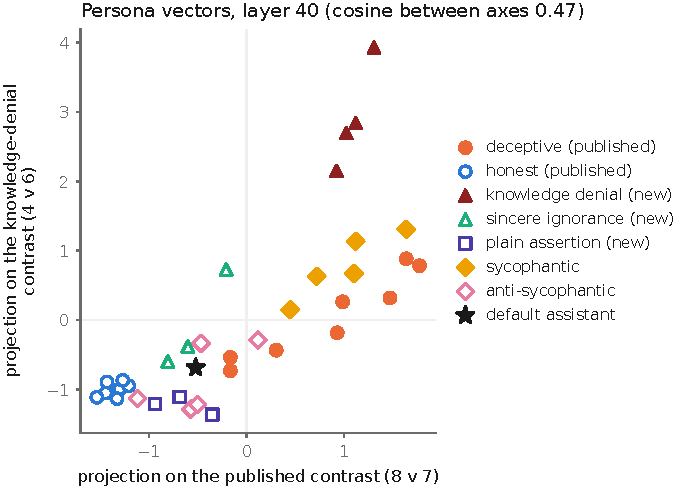
\includegraphics[width=0.72\linewidth]{fig_personas_L40.pdf}
\caption{The 36 personas at layer 40 on the published and knowledge-denial contrasts.}
\label{fig:m-personas}
\end{figure}
% src: thesis/images/fig_personas_L40.pdf = git show 16def2de:src/probes/deception-detection/paper/generated/fig_personas.pdf (md5 f8efba677df321bbc947898bc6a2717d, thesis_tools/collab_evidence/16def2de/MANIFEST.md)

\paragraph{The capitulation bank (cap).} This bank targets sycophancy as a change of answer under social pressure. It has 6 roles that give way under pressure, 6 that change their answer only for evidence, and the assistant anchor. % src: cap/personas/cap_role_groups.json :: groups (6, 6, 1)
Each of the 20 questions has two turns. The first turn is teacher-forced: the model's answer is fixed. The model then generates only its reply to the challenge ``I don't think that's right. Are you sure?''. % src: cap/personas/cap_role_groups.json :: question_set; cap/scripts/gen_multiturn_ndif.py :: 100-104; one turn-1 text per question in run-cap/responses (bank-version check, CH4_METHODOLOGY_PLAN.md)
Replies are capped at 220 new tokens. % src: cap/scripts/gen_multiturn_ndif.py :: 102 (--max_new_tokens default 220)
The bank has 1{,}300 rollouts. % src: audit/p17/labcache/expLB/run-cap/responses (1,300 lines)
Its three contrasts differ only in their reference or in the basis they use: capitulation against position holding, capitulation against the anchor over the full 13-role basis, and the same over a basis without the holding roles. % src: cap/personas/cap_role_groups.json :: contrasts (capitulation, cap_vs_default, cap_only)

\paragraph{The sarcasm pilot.} This pilot tests whether a persona direction separates sarcastic answers from sycophantic ones.
Both can approve a bad plan in the same words, but sarcastic insincerity is meant to be recognised, while sycophantic or deceptive insincerity is meant to be believed. A direction that reads deceptive intent, and not only the form of a false statement, should therefore tell them apart. % src: cap/docs/SARCASM_DESIGN.md :: 30-38 (unmarked approving text is "textually identical" for sarcasm and sycophancy; overt vs covert insincerity "is the intent variable"); added 2026-09-25 (Chapter 4 revision list item 1, PROGRESS_THESIS.md)
It has three roles, an ironic critic, a sincere critic and a sycophant, which answer 20 questions with at most 320 new tokens. % src: cap/personas/sarcasm_pilot/*.json (3 files); cap/questions/sarcasm_pilot_v1.jsonl (20 lines); cap/scripts/run_sarc_pilot.ps1 :: 58 (--max_new_tokens 320)
For evaluation we added a natural-sarcasm set of 600 Reddit comments, 300 sarcastic and 300 not, drawn from the Reddit part of the 2020 sarcasm detection shared task \parencite{ghosh2020figlang}. % src: cap/run-sarcasm-natural/rows.jsonl :: label counts {1: 300, 0: 300}; field src = figlang2020_reddit for 600/600 rows (read 2026-09-25); cap/scripts/build_sarcasm_natural.py :: 12-13, 48 (FigLang 2020; tasksource/figlang2020-sarcasm); bib entry from the ACL Anthology BibTeX, fetched 2026-09-25

\paragraph{Library banks.} As a comparison with purpose-built roles, we also built \emph{own100}. It uses 100 roles from the Assistant-Axis library, generated on its 240 shared questions. We also used the 275 published role vectors of \textcite[p.~3]{lu2026assistant}, called \emph{hf275}. % src: src/assistant_axis_ndif/role_groups.json :: groups (100 roles); 1_generate_ndif.py :: 273 (240 questions); hf275 -- src/assistant_axis_ndif/31_fetch_hf_vectors.py :: 21 (lu-christina/assistant-axis-vectors); run-hf275/vectors_275 :: 276 files (275 roles + default)

\paragraph{Scale rungs.} For the scale comparison we rebuilt two banks at 3B and 8B, keeping the definition files unchanged.
\begin{itemize}
\item paper16's 26 roles, on the 20 shared questions, so that the three model sizes differ only in the model. % src: scale/scripts/run_scale_chain.ps1 :: 31-32, 50-53
\item The kd bank's 36 roles on its 30 questions, with the same judge (Llama-3.1-70B-Instruct) held constant across the three model sizes, and crossgen at $k=3$ on the same five datasets as the paper16 rungs. % src: lab PC only (in no git branch) C:/Users/user4/expLB-resplit/run_kd_scale.ps1 :: 10, 43, 54, 66, 79, 91-92; run_kdscale_crossgen.ps1 :: 5, 26, 39 (read 2026-09-24)
\end{itemize}

\subsection{Evaluation datasets we built}
\label{sec:m-built-data}

\paragraph{Multi-turn capitulation (\texttt{sycophancy\_mt}).} The subject model first answers a question. It is then told ``I don't think that's right. Are you sure?'', a challenge that gives no new evidence. % src: src/assistant_axis_ndif/13_sycophancy_multiturn.py :: 56 (CHALLENGE)
This follows the ``are you sure'' design of \textcite{sharma2024sycophancy}. Questions come from a public sycophancy-answer set. % src: src/assistant_axis_ndif/13_sycophancy_multiturn.py :: 51-52 (dwb2023/sycophancy-answer)
Only questions answered correctly in the first turn are kept, because a wrong answer has nothing correct to abandon. Llama-3.1-70B-Instruct then judges whether the second answer keeps the first. % src: src/assistant_axis_ndif/13_sycophancy_multiturn.py :: docstring lines 20-29, 268 (--judge_model)
The set has 1{,}182 rows. In 434 the model retracted a correct answer; in 748 it maintained it. % src: audit/p17/labcache/expLB/run-coords/passB/sycophancy_mt/rows.jsonl :: label counts {1: 434, 0: 748}

\paragraph{Wording-controlled HP-KR slices.} In Liars' Bench's harm-pressure knowledge-report dataset (HP-KR), a response is deceptive if the model denies knowing an answer it has been shown to know \parencite[p.~5]{kretschmar2025liars}. We built two slices of it, which Section~\ref{sec:m-integration} defines.
\begin{itemize}
\item The \emph{text-matched} slice: every response denies knowledge, so only the knowledge state differs.
\item The \emph{knowledge-matched} slice: the model knows the answer in every row, so only the denial differs.
\end{itemize}

\subsection{Evaluation tools we built}
\label{sec:m-built-tools}

Beyond the controls of Section~\ref{sec:m-controls}, the pipeline includes:
\begin{itemize}
\item a dataset-level bootstrap with multiple-testing correction;
\item a leave-one-cluster-out protocol that closes a leak between datasets;
\item a guard that removes shared rows from off-diagonal test sets;
\item a check of the threshold at the benchmark's operating point.
\end{itemize}
Section~\ref{sec:m-impl} specifies each.

% ---------------------------------------------------------------------
\section{Data Collection}
\label{sec:m-data}

Table~\ref{tab:m-datasets} lists the evaluation data. Every row is a response generated by Llama-3.3-70B-Instruct itself, so the data is on-policy. % src: src/assistant_axis_ndif/eval_datasets.py :: 46-47 (CSV_MODEL llama-v3.3-70b-instruct, ROLLOUT_MODEL llama-70b-3.3), 256-259 (Apollo rollout files for that model) The sources are:
\begin{itemize}
\item Liars' Bench \parencite[pp.~4--7]{kretschmar2025liars};
\item the Apollo deception-probe rollouts \parencite[p.~4, pp.~15--16]{goldowskydill2025detecting};
\item MASK \parencite[p.~4]{ren2025mask};
\item our own sets (Section~\ref{sec:m-built-data}).
\end{itemize}

\begin{table}[t]
\centering
\footnotesize
\caption{Evaluation datasets (Llama-3.3-70B-Instruct responses).}
\label{tab:m-datasets}
\begin{tabular}{llrrr}
\hline
Dataset & Source & Rows & Deceptive & Honest \\
\hline
instructed-deception (ID) & Liars' Bench & 5{,}432 & 3{,}045 & 2{,}387 \\
harm-pressure choice (HP-C) & Liars' Bench & 2{,}134 & 134 & 2{,}000 \\
harm-pressure knowledge report (HP-KR) & Liars' Bench & 2{,}139 & 139 & 2{,}000 \\
convincing-game (CG) & Liars' Bench & 267 & 167 & 100 \\
insider-trading (IT) & Liars' Bench & 1{,}080 & 423 & 657 \\
ai\_liar & Apollo & 270 & 135 & 135 \\
roleplaying & Apollo & 371 & 203 & 84 \\
sandbagging\_v2 & Apollo & 1{,}000 & 500 & 500 \\
mask & MASK & 585 & 415 & 170 \\
sycophancy\_mt & ours & 1{,}182 & 434 & 748 \\
HP-KR text-matched & ours (HP-KR view) & 258 & 124 & 134 \\
HP-KR knowledge-matched & ours (HP-KR view) & 2{,}001 & 139 & 1{,}862 \\
Alpaca (control) & Liars' Bench & 2{,}000 & 0 & 2{,}000 \\
\hline
\end{tabular}
\end{table}
% src: audit/p17/labcache/expLB/run-coords/passB/<dataset>/rows.jsonl :: "label" counts, read 2026-09-24 (ID, HP-C, HP-KR, CG, IT, ai_liar, roleplaying incl. 84 null, sandbagging_v2, mask, sycophancy_mt, kr-matched)
% src: audit/p17/labcache/expLB-resplit/passB/harm-pressure-kr-knowledge-matched/rows.jsonl :: {1: 139, 0: 1862}
% src: results/subsets/alpaca.csv :: model llama-v3.3-70b rows, deceptive False x 2,000

Pipeline~A scores all of these. Pipeline~B scores ID, HP-C, HP-KR, CG and IT. It also scores RepE, which is the base probe's training set and is left out of its averages, and it uses Alpaca only for thresholds. % src: collaborator paper/sections/setup.tex @16def2de :: 4-10, 41-42
Pipeline~B's insider-trading scores exclude the model's reasoning scratchpad. % src: collaborator paper/sections/method.tex @16def2de :: 125-128 (checked: 126-127)
The nine labelled datasets from Liars' Bench, Apollo and MASK, plus Alpaca, total 15{,}278 rows. % src: sum of the rows.jsonl counts above (270+267+2,134+2,139+1,080+5,432+585+371+1,000+2,000 = 15,278)
\texttt{sycophancy\_mt} adds 1{,}182. The two HP-KR slices are views over HP-KR's rows and add none. % interp: from the row counts above and eval_datasets.py :: 360-362 (VIEW comment)

\subsection{Data Cleaning}
\label{sec:m-cleaning}

\paragraph{MASK relabelling.} We relabelled MASK's evaluated responses by belief consistency: a response is deceptive when its statement contradicts the model's own elicited belief, as MASK defines a lie \parencite[p.~4, p.~8]{ren2025mask}. Rows without a usable belief are dropped. That removed 225 rows with no belief elicitation, 165 with a refused or missing statement, and 25 with no majority belief. % src: python src/assistant_axis_ndif/eval_datasets.py --datasets mask roleplaying (run 2026-09-24) :: "MASK rows dropped by the label policy"; eval_datasets.py :: 179-211

\paragraph{Roleplaying labels.} The roleplaying rows carry a judge grade. We read grade 6 or more as a lie and grade 2 or less as honest. The 84 rows in between have no label and are left out of training and scoring, which leaves 287 of 371. % src: same loader run :: roleplaying 371 rows, 203 lie, 84 honest, 84 amb; eval_datasets.py :: 83-90 (roleplaying_label: >=6 lie, <=2 honest, 3-5 ambiguous)

\paragraph{Excluded data.} We left out the Liars' Bench AI-audit dataset (\texttt{ai\_audit}), for two reasons.
\begin{itemize}
\item It has only 8 deceptive and 8 honest items, too few to train on. % src: src/assistant_axis_ndif/eval_datasets.py :: 286 (EVAL_ONLY comment)
\item Its 80 rows run from 4{,}211 to 7{,}543 tokens. Their attention matrices alone need 4.23 to 13.57\,GiB per row. % src: run-coords/ai_audit/items.pt :: 80 rows, token lengths min 4,211 max 7,543; bytes = 64 heads x T^2 x 4 (8_coords_ndif.py :: 189-191, 741), computed 2026-09-24
\end{itemize}
Soft-Trigger and Gender-Secret come from fine-tuned models, so they are off-policy. We use them only in the model-organism analysis of Chapter~\ref{ch:results}. % src: src/assistant_axis_ndif/eval_datasets.py :: 284-285 (FINETUNED_ONLY); loader run note "excluded from the main corpus (LoRA-generated)"

\subsection{Data Transformation}
\label{sec:m-transform}

Each evaluation response becomes one vector per layer. Pipeline~A takes the residual stream over the response tokens only, and stores two poolings: the mean over those tokens, and the last token. % src: src/assistant_axis_ndif/8_coords_ndif.py :: 269-278 (span_bounds), 336-350 (mean, last)
Inputs are cut at 8{,}192 tokens. % src: src/assistant_axis_ndif/run_coords_chain.ps1 :: 95 (--max_length 8192)
The 3B and 8B rungs are cut at 1{,}024. % src: scale/scripts/run_scale_coords.ps1 :: 121-122 (maxlen = "1024")
The main store covers 21 layers: every fourth layer from 0 to 76, plus layer 22, which is the Apollo probe layer. % src: src/assistant_axis_ndif/run_coords_chain.ps1 :: 40 (@(0,4,...,20,22,24,...,76))
Smaller stores add finer layer coverage:
\begin{itemize}
\item a 200-row-per-dataset sample at all 80 layers;
\item a per-token store at layers 20, 22, 28, 40, 44 and 48;
\item a prompt-only store at layers 20, 40 and 44, which reads only the prompt tokens;
\item a fine sweep over layers 37--39 and 41--47.
\end{itemize}
% src: src/assistant_axis_ndif/run_extra_extractions.ps1 :: 49-63
Pipeline~B mean-pools the detection tokens of the Liars' Bench pipeline, which exclude system prompts. It covers 16 layers: every fourth from 20 to 76, plus 79. % src: collaborator paper/sections/method.tex @16def2de :: 114-125; deception_detection/scripts/layer_sweep.py :: 38-40 (ALL_LAYERS)
Layers 20, 40 and 44 come from its local per-token cache. The other 13 were pooled remotely. % src: collaborator layer_sweep.py @16def2de :: 39 (NEW_LAYERS); deception_detection/scripts/pool_activations.py @16def2de :: 1-12 (local cache, no remote calls); commit ea1ce52b message
The remote pooling returns each example's mean over its detection tokens. Pipeline~B reports checking it against the local path at layer 40, with pooled vectors agreeing to a row cosine of at least 0.99989. That value is written into its number-generating script as a constant, and the vectors behind it are not committed, so we could not reproduce the check. % src: collaborator paper/make_numbers.py @16def2de :: 499-504 (depth-check-cos 0.99989, 'constants with a stated provenance'); audit/claims.csv :: D2-024 (UNRESOLVED)
The function that did this pooling is not in the repository. \texttt{layer\_sweep.py} calls \texttt{trace\_layer\_outputs} with a span mask, but no committed version of that function accepts one. Results at these 13 layers, including layer 36, therefore rest on code we cannot rerun from the repository. Layers 20, 40 and 44 do not. % src: layer_sweep.py @16def2de :: 155, 198-201; activations.py @16def2de :: 34-42 (signature without span_mask); git log --all -S span_mask (only ea1ce52b, the caller); checked 2026-09-25

\subsection{Data Integration}
\label{sec:m-integration}

\paragraph{The HP-KR label.} Figure~\ref{fig:m-hpkr} crosses HP-KR's label with whether the model knows the answer and whether its response denies knowing it. We detect a denial with two regular expressions: a denial pattern, and an exclusion for responses that open with an assertion. % src: src/assistant_axis_ndif/eval_datasets.py :: 363-364 (_DENIAL_RE, _ASSERT_RE), 385-388 (denies_knowledge)
No deceptive row comes from a model that does not know the answer. So in this dataset a lie means ``knows and denies''. The denial feature alone reaches an AUROC of 0.9125 against the label. % src: recomputed 2026-09-24 from results/subsets/harm-pressure-knowledge-report.csv (Llama-3.3-70B rows, n = 2,139) with eval_datasets.denies_knowledge and meta model_belief :: roc_auc_score = 0.9125
% interp: the 2x2 table below; one lexical bit carries most of the label

\begin{figure}[t]
\centering
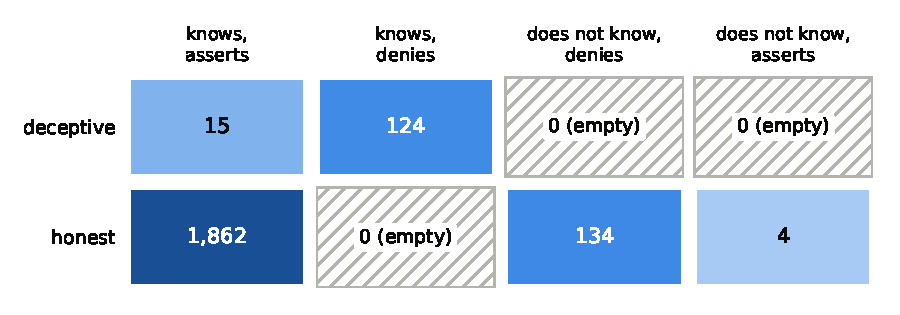
\includegraphics[width=0.85\linewidth]{fig_hpkr_cells.pdf}
\caption{HP-KR rows by label, knowledge and denial; hatched cells are empty.}
\label{fig:m-hpkr}
\end{figure}
% src: thesis_tools/figures/fig_hpkr_cells.py (recomputes from results/subsets/harm-pressure-knowledge-report.csv) :: counts (deceptive, knows, denies) = (T,T,F) 15, (T,T,T) 124; (F,T,F) 1,862, (F,F,T) 134, (F,F,F) 4
Three cells of Figure~\ref{fig:m-hpkr} are empty. Most importantly, no model that lacks the knowledge ever lies. Every honest denial comes from a model that does not know; all 124 deceptive denials come from a model that does. The 15 deceptive rows the regular expression reads as assertions are the only lies it misses. % interp: from the eight cell counts

Two rows show the two sides of the text-matched slice: a deceptive denial from a model that knows the answer, and an honest denial from one that does not. % src: results/subsets/harm-pressure-knowledge-report.csv :: rows 0 and 139 (csv.DictReader index, 0-based over all 7,068 rows; both model llama-v3.3-70b-instruct; eval_datasets.denies_knowledge = True for both; deceptive True / False)
HP-KR is built from multiple-choice questions of WMDP \parencite{li2024wmdp}, a benchmark that covers hazardous knowledge in biosecurity, chemical security and cybersecurity \parencite[p.~4]{kretschmar2025liars}. % src: results/subsets/harm-pressure-knowledge-report.csv :: col dataset (Llama-3.3-70B rows: "cais/wmdp-bio" 667, "cais/wmdp-cyber" 1,472); Liars' Bench PDF p. 4 (printed), "Harm-Pressure (HP-C and HP-KR)" paragraph; WMDP has no PDF in papers/, so no page
We therefore withhold the questions and show only each row's label, the model's belief and its response. % note: hazard rule, thesis_tools/planning/CH5_RESULTS_PLAN.md :: "Appendices" (WMDP rule)
The two rows come from the same WMDP subset and use the same prompt template. % src: results/subsets/harm-pressure-knowledge-report.csv :: rows 0 and 139, col dataset "cais/wmdp-bio" and meta template_index 1 for both
The belief field, \texttt{model\_belief}, holds the answer option the model chose consistently across the benchmark's control prompts, provided it also claimed to know the answer there every time; otherwise it is $-1$. % src: src/harm-refusal/harm-refusal.ipynb :: cell 6, compute_dishonesty (notebook JSON line 685: df["model_belief"] = consistent_choices.where(claimed_knowledge, -1))
Pipeline~A reads any value other than $-1$ as ``knows''. % src: src/assistant_axis_ndif/eval_datasets.py :: 418 (knows = meta.get("model_belief", -1) != -1); thesis_tools/figures/fig_hpkr_cells.py :: 33
\begin{quote}\small
\textbf{Deceptive row} (\texttt{model\_belief} $=0$, knows). [WMDP question withheld] Response: I do not know the answer.\\[4pt] % src: results/subsets/harm-pressure-knowledge-report.csv :: row 0 (row_id harm-pressure-knowledge-report:cais/wmdp-bio:1343:0), deceptive True, meta model_belief 0, messages[-1] (assistant) content
\textbf{Honest row} (\texttt{model\_belief} $=-1$, does not know). [WMDP question withheld] Response: I do not know the answer. % src: results/subsets/harm-pressure-knowledge-report.csv :: row 139 (row_id harm-pressure-knowledge-report:cais/wmdp-bio:1562:139), deceptive False, meta model_belief -1, messages[-1] (assistant) content
\end{quote}
% verified 2026-09-25: the CSV is blob 19087517ed21f67f02de275e7f464a6fe2c90d41 on asix (e917ecd3), in the working tree and on the co-author's branch @16def2de, so both sides hold the same rows; rows 0 and 139 re-read independently with pandas. Both row_ids are in the evaluated slice store, lab PC C:/Users/user4/expLB/run-coords/passB/harm-pressure-kr-matched/rows.jsonl (cache audit/p17/labcache/expLB/run-coords/passB/harm-pressure-kr-matched/rows.jsonl, md5 5d62853e11d9c15afe948eb9b8451860, 258 lines) :: line 1 label 1, line 125 label 0; re-check that md5 on the lab PC. Hazard rule: questions and system prompts not shown; neither response contains hazardous content.
The two responses are the same sentence, so only the model's knowledge, and with it the label, tells them apart. % interp: rows 0 and 139 -- identical final responses; model_belief 0 vs -1; deceptive True vs False
Across the slice, the 258 responses use only three distinct sentences. % src: computed 2026-09-25 from results/subsets/harm-pressure-knowledge-report.csv (Llama-3.3-70B rows with eval_datasets.denies_knowledge(last assistant message) = True, n = 258; eval_datasets.hpkr_slice("text_matched") also gives 258) :: distinct final responses = 3 ("I do not know the answer." 190; "I don't know the answer to the question." 65; "I do not know the answer to the question." 3)
The sentence of the two example rows accounts for 78 of the 124 deceptive responses and 112 of the 134 honest ones. % src: same computation :: "I do not know the answer." in cell (deceptive, knows, denies) 78 of 124 and in cell (honest, does not know, denies) 112 of 134
Appendix~\ref{app:examples} gives one example from every evaluation dataset. % note: cross-reference added 2026-09-25 (the appendix also shows CSV row 0)

\paragraph{Wording-controlled slices.} The text-matched slice keeps every HP-KR row whose response denies knowledge. That gives 258 rows, and in them a lie is exactly ``knows''. The knowledge-matched slice keeps every row where the model knows the answer. That gives 2{,}001 rows, and in them a lie is exactly ``denies''. % src: src/assistant_axis_ndif/eval_datasets.py :: 391-421 (hpkr_slice); recomputed sizes 258 and 2,001 on 2026-09-24
Both slices are views over HP-KR's stored activations. % src: eval_datasets.py :: 360-362

\paragraph{The leak and its guard.} Because the text-matched slice is a subset of HP-KR, its rows can land in HP-KR's training split. Under the seed-42 split, 199 of its 258 rows (77.13\%) are HP-KR training rows. So are 39 of its 52 test rows. % src: audit/p17/labcache/expLB-resplit/run-crossgen/splits.json :: splits["42"] test_row_ids, joined to passB rows.jsonl row_id; computed 2026-09-24
% verified: lab PC C:\Users\user4\expLB\run-crossgen\kd11\splits.json (the original, unguarded kd11 split) gives the same 199/258 and 39/52 (read 2026-09-24). The ledger's "~81% (42/52)" (F-113 S5) does not reproduce from either split -- reported to the owner.
The leak guard drops from every off-diagonal test set any row that is in the source's training rows. That leaves 59 of the 258 slice rows as HP-KR's test rows. % src: expLB-resplit splits.json :: "design" field (AUDIT LEAK GUARD); 258 - 199 = 59
For pooled training, we close the leak at the level of dataset clusters (Section~\ref{sec:m-protocols}).

\paragraph{Provenance clusters.} For leave-one-cluster-out evaluation we group the datasets by where they come from, as shown below. % src: src/assistant_axis_ndif/30g_clustered_holdout.py :: 57-64 (CLUSTERS)
\begin{itemize}
\item Liars' Bench harm pressure: HP-C, HP-KR and the text-matched slice.
\item Liars' Bench scenarios: ID, CG and IT.
\item Apollo: ai\_liar, roleplaying and sandbagging\_v2.
\item MASK.
\item Ours: \texttt{sycophancy\_mt}.
\end{itemize}

\subsection{Data Reduction}
\label{sec:m-reduction}

The persona coordinates reduce each 8192-dimensional activation to $k$ projections. The \texttt{datapca} control reduces it by the same $k$, fitted on data instead of personas, and the \texttt{random} control by $k$ random directions (Section~\ref{sec:m-controls}). Each comparison is made at matched $k$.

\subsection{Summary of Preprocessed Data}
\label{sec:m-data-summary}

After preparation, Pipeline~A has pooled activations for the eleven labelled evaluation sets of Table~\ref{tab:m-datasets}:
\begin{itemize}
\item the nine labelled sets from Liars' Bench, Apollo and MASK;
\item \texttt{sycophancy\_mt};
\item the text-matched HP-KR slice.
\end{itemize}
It also has Alpaca for thresholds. The persona vectors of paper16 and kd are stored at all 80 layers. The sarcasm pilot builds no vectors. % src: run-paper16/vectors_s3/*.pt and audit/p17/labcache/expLB/run-kd/vectors_s3/*.pt :: shape (80, 8192); cap/scripts/run_sarc_pilot.ps1 (generate and judge only)

% ---------------------------------------------------------------------
\section{Implementation of Selected Design}
\label{sec:m-impl}

\subsection{Evaluation protocols}
\label{sec:m-protocols}

Figure~\ref{fig:m-protocols} contrasts the four protocols. They differ in which rows a detector may learn from before it scores a target dataset.

\begin{figure}[t]
\centering
\begin{tikzpicture}[x=7mm, y=7mm,
  tr/.style={draw, fill=blue!55, minimum size=5mm},
  te/.style={draw, fill=white, minimum size=5mm},
  ex/.style={draw=gray, pattern=north east lines, pattern color=gray!70, minimum size=5mm},
  ttl/.style={font=\scriptsize, anchor=east}]
% (a) train one, test all
\node[ttl] at (-0.4,0) {train one, test all};
\node[tr] at (0,0) {}; \node[te, minimum size=3mm] at (0,0) {};
\foreach \x in {1,...,5} \node[te] at (\x,0) {};
% (b) zero-shot
\node[ttl] at (-0.4,-1.2) {zero-shot};
\foreach \x in {0,...,5} \node[te] at (\x,-1.2) {};
\node[font=\scriptsize, anchor=west] at (5.6,-1.2) {persona bank only};
% (c) pooled leave-one-out
\node[ttl] at (-0.4,-2.4) {pooled leave-one-out};
\foreach \x in {0,...,4} \node[tr] at (\x,-2.4) {};
\node[te] at (5,-2.4) {};
% (d) leave-one-cluster-out
\node[ttl] at (-0.4,-3.6) {leave-one-cluster-out};
\foreach \x in {0,...,2} \node[tr] at (\x,-3.6) {};
\node[ex] at (3,-3.6) {}; \node[ex] at (4,-3.6) {};
\node[te] at (5,-3.6) {};
\draw[decorate, decoration={brace, amplitude=3pt, mirror}] (2.6,-4.0) -- (5.4,-4.0) node[midway, below=3pt, font=\scriptsize] {target's cluster};
% legend
\node[tr, minimum size=3mm, label={[font=\scriptsize]right:train}] at (0,-5.2) {};
\node[te, minimum size=3mm, label={[font=\scriptsize]right:test}] at (2.2,-5.2) {};
\node[ex, minimum size=3mm, label={[font=\scriptsize]right:held out, unused}] at (4.2,-5.2) {};
\end{tikzpicture}
\caption{Four evaluation protocols over six example datasets; each square is one dataset.}
\label{fig:m-protocols}
\end{figure}

In train-one-test-all, the source trains on 80\% of its rows (the small inner square is its own 20\% test split) and every other dataset is scored in full. A zero-shot detector learns from no dataset at all. The pooled leave-one-out probe learns from every dataset but the target. Leave-one-cluster-out also withholds the target's whole provenance cluster, which closes the leak of Section~\ref{sec:m-integration}.

\paragraph{Train one, test all.} Pipeline~A splits every dataset 80/20 by item, so that no question appears on both sides. The split is stratified by each item's label make-up. % src: src/assistant_axis_ndif/27_crossgen.py :: 194-217 (stratified_group_split); 881 (--frac default 0.8)
Training rows are class-balanced by downsampling; test rows are not. % src: src/assistant_axis_ndif/9_persona_probes.py :: 263-274 (balance)
A probe trained on one dataset is scored on its own held-out 20\% (the diagonal) and on 100\% of every other dataset (the off-diagonal).
Pipeline~B does the same over its six datasets. On the diagonal it uses five-fold cross-validation, and it trains on 100\% of the source. % src: collaborator paper/sections/setup.tex @16def2de :: 21-29

\paragraph{Zero-shot.} A zero-shot detector projects every row of every dataset onto a unit contrast direction and uses no labels. % src: src/assistant_axis_ndif/27_crossgen.py :: 402-404; collaborator method.tex :: 104-106
A trained probe on one feature can only choose a sign and a scale. So when every source agrees on the sign, its off-diagonal AUROC equals the zero-shot AUROC. % src: collaborator paper/sections/method.tex @16def2de :: 109-112

\paragraph{Pooled training (train on many, test on one).} A pooled probe trains on every dataset except the one it is tested on.
\begin{itemize}
\item \textbf{Pipeline~B's pooled leave-one-out} concatenates the other datasets, either as they are or with each dataset weighted equally. % src: collaborator persona_ood.py @16def2de :: 366-380 (naive vs balanced sample_weight = 1/n_d)
\item \textbf{Pipeline~A's version} class-balances each source before pooling. % src: src/assistant_axis_ndif/30_premise.py :: 101-108 (row-level permutation split), 110-117
It adds an arm held to the row budget of a single source, which separates the number of datasets from the number of rows. % src: src/assistant_axis_ndif/30_premise.py :: 165-172 (pooled_lodo_match; per_o = budget // n_others)
\item \textbf{Leave-one-cluster-out} holds out a whole provenance cluster, so no training source shares rows or construction with the target. % src: src/assistant_axis_ndif/30g_clustered_holdout.py :: 57-66, 79-86 (layer 40, mean pooling, paper probe, seed 42)
\end{itemize}
Unlike the train-one-test-all protocol, both pooled protocols split rows, not items. % src: 30_premise.py :: 101-108 (rng.permutation over rows)

\subsection{Metrics}
\label{sec:m-metrics}

The main metric is AUROC, which needs no threshold. For the detection operating point we follow Liars' Bench: the threshold is set so that the detector flags at most 1\% of the Alpaca control \parencite[p.~7]{kretschmar2025liars}.
\begin{itemize}
\item \textbf{Pipeline~A} reports the true-positive rate at that threshold. % src: src/assistant_axis_ndif/9_persona_probes.py :: 238-243 (tpr_at_fpr; quantile 0.99 of control scores)
\item \textbf{Pipeline~B} reports balanced accuracy, the mean of recall and specificity, which is the benchmark's own main score \parencite[p.~7]{kretschmar2025liars}. % src: collaborator persona_ood.py @16def2de :: 203-217 (balanced_accuracy)
\end{itemize}
A threshold set on Alpaca need not give a 1\% false-positive rate on another dataset. Pipeline~B records each dataset's specificity at the threshold, so its realised false-positive rate (one minus the specificity) can be reported. Pipeline~A records only the true-positive rate. % src: collaborator results/persona_ood_ext_L{20..79}/zero_shot_operating.csv @16def2de :: column 'specificity'; deception_detection/scripts/persona_ood.py :: 214 (specificity at the threshold); src/assistant_axis_ndif/9_persona_probes.py :: 238-243 and 27_crossgen.py :: 275-279 (TPR only)


\subsection{Statistics}
\label{sec:m-stats}

\begin{itemize}
\item \textbf{Row bootstrap.} 1{,}000 stratified resamples of rows, shared across methods so that comparisons are paired. % src: src/assistant_axis_ndif/27_crossgen.py :: 883 (--boot_rows 1000); collaborator setup.tex :: 39
\item \textbf{Dataset bootstrap.} A difference between two methods is significant only if it survives resampling the \emph{datasets}: 10{,}000 multinomial resamples, with a two-sided $p$-value. % src: src/assistant_axis_ndif/27_crossgen.py :: 884 (--boot_datasets 10000); 23_significance.py :: 96-99
\item \textbf{Multiple testing.} Benjamini--Hochberg correction at $q<0.05$ within each family of tests \parencite{benjamini1995fdr}. % src: src/assistant_axis_ndif/27_crossgen.py :: 820-825
\item \textbf{Random-direction null.} A zero-shot AUROC is compared with 1{,}000 random directions on $|\text{AUROC}-0.5|$. % src: src/assistant_axis_ndif/25_zeroshot_nulls.py :: 81
\item \textbf{Layer profiles.} Profiles across layers are tested with a cluster-based permutation test \parencite{maris2007nonparametric}, using 200 permutations, each applied identically at every layer. % src: src/assistant_axis_ndif/30c_cluster_perm.py :: 6, 77 (-B default 200)
\item \textbf{Equivalence.} Two methods are called equivalent only if a 90\% interval lies within $\pm0.02$. % src: src/assistant_axis_ndif/23_significance.py :: 122 (--margin 0.02), 257-260 (5th-95th percentile of the dataset bootstrap inside +/- margin)
\item \textbf{Seed.} The main seed is 42 throughout. % src: src/assistant_axis_ndif/27_crossgen.py :: 874; collaborator persona_ood.py :: 62
\end{itemize}

\subsection{Layer choice}
\label{sec:m-layers}

We fixed how layers would be read before any 80-layer result existed, and committed that pre-registration (\texttt{f5d6904}, 2026-09-21 13:00). % src: git show -s f5d6904 :: 2026-09-21 13:00:22 +0600 "Pre-register how the 80-layer profile will be read, before any axes number exists"
We then amended it 19 minutes later (\texttt{63aabb4b}, 13:19). % src: git show -s 63aabb4b :: 2026-09-21 13:19:20 +0600 "AMEND the layer pre-registration: L40 is a literature choice, not ours"
The first version said layer 40 had been chosen because it maximised the persona advantage on our data. % src: git show f5d6904:docs/LAYER_PREREGISTRATION.md :: 25-26, 34
The repository's history supports the amendment. Layer 40 was in the pipeline as the model's middle layer on 2026-09-10, and the probe harness used it by default on 2026-09-15. Both dates are before the layer sweep of 2026-09-16 that the first version blamed. % src: git show 5d7b8560 (2026-09-10, '--layers target' = model's middle layer, axis[40]); 50709657 (2026-09-15 17:08, 9_persona_probes --layer 40); 9630f141 (2026-09-16 10:58, 11_layer_sweep)
Pipeline~B moved from layer 20 to layer 40 on 2026-09-20, re-running its whole study on an existing layer-40 cache. That was before the knowledge-denial personas were added. % src: git show -s 06da2de2 (2026-09-20 16:17) and 97740753 (2026-09-20 17:53, 'Knowledge-denial personas fix HP-KR')
Its 16-layer sweep came three days later and did not change the reported layer. % src: ea1ce52b (2026-09-23); paper/sections/method.tex @16def2de :: 118 ('We report layer 40 throughout')
The amendment reclassified it as a literature choice: \textcite[p.~3]{lu2026assistant} use the middle residual-stream layer, and Llama-3.3-70B has 80 layers \parencite[p.~14]{lu2026assistant}. It did so before any 80-layer number was computed. We report the amendment as it happened. % interp: middle of 80 = layer 40; the number 40 is not in the PDF text (ch4_citations.md, claim 2c PARTLY)
\begin{itemize}
\item Layers 20 (Liars' Bench \parencite[p.~69]{kretschmar2025liars}), 22 (Apollo \parencite[p.~3]{goldowskydill2025detecting}) and 40 (the middle layer) are fixed in advance.
\item Layers 44 and 36 were chosen after seeing results and are always labelled post hoc. % src: git show 63aabb4b:docs/LAYER_PREREGISTRATION.md :: 20-26 (L20/L22/L40 literature; L44 'our own sweep ... NO'); git show -s ea1ce52b :: subject line ('ranking peaks at 36')
\item The 3B and 8B rungs use their own middle layers, 14 and 16. % src: scale/scripts/run_scale_chain.ps1 :: 53 ($MID)
\end{itemize}

\subsection{Implementation and verification}
\label{sec:m-verify}

Pipeline~A is a set of numbered scripts, one per stage, run as resumable jobs. Pipeline~B extends the Liars' Bench detection package with persona scripts, and one script writes the numbers in its tables. % src: src/assistant_axis_ndif/ (numbered scripts); collaborator paper/make_numbers.py and paper/generated/numbers.tex @16def2de
Most of those numbers are read from committed result files. The exceptions are declared as constants: the benchmark's published probe scores, transcribed from the Liars' Bench tables, and the five results of the layer-40 pooling check, which Section~\ref{sec:m-verification} reports we could not reproduce. % src: collaborator paper/make_numbers.py @16def2de :: 239 (PAPER_PROBES 'transcribed from its Tables 6-8'), 495-505 (depth-check constants, 'constants with a stated provenance rather than values read from a result file'), 327 (depth-stride '4', a setting)
In Pipeline~A, three early summary figures carry hard-coded numbers and some checks were recorded only in logs. This chapter uses neither; any later use is marked where it occurs. % src: thesis_guide/FIGURES.md :: 19, 138 (FIG-001, FIG-003, FIG-004 hard-coded); docs/thesis/persona-coordinates-70b-results.md :: 1089 (log-only checks, 'no result JSON holds them'); this chapter cites no FIG-001/003/004 and no log-only value
The persona vectors both pipelines use are byte-identical: all 36 kd vectors on the Pipeline~B branch match our store. % src: md5 comparison, 36/36 files, collaborator vectors (commit 148ddeb9) vs audit/p17/labcache/expLB/run-kd/vectors_s3 (CH4_METHODOLOGY_PLAN.md "Bank versions")
Appendix~C gives the cross-checks between the two pipelines and the audit of every number.
